\chapter{The Standard Model}\label{ch:sm}

\newcommand{\ct}{\cos\theta_w}
\newcommand{\st}{\sin\theta_w}

In this chapter we will describe the components of the Standard Model (SM) of particle physics, with particular attention to the theory of weak interactions. The treatment is semi-historical. We assume familiarity with the basic concepts of quantum field theory and quantum electrodynamics (\textsc{qed}), including what a particle is, the connection between particles and fields, and how to interpret Feynman diagrams. For a refresher on group theory concepts, one may turn to \autoref{ch:qft}. We will first talk about the matter content, followed by a discussion of gauge invariance and how it leads to gauge fields that both interact with themselves and mediate the interactions between the matter fields. We then discuss the historical development of electroweak theory, and build up to an explanation of electroweak symmetry breaking and the Higgs mechanism. Strong interactions and the concept of asymptotic freedom are briefly discussed, after which We conclude by highlighting the limits of the Standard Model and the need for new physics extensions to it. The material in this chapter draws from a number of excellent treatments of the subject \citep{Cheng1985,Schwartz2014,Zee2010,Peskin:1995ev}.

\section{Particle content}

The fundamental constituents of matter are fermions. They come in two varieties - quarks and leptons. Quarks are found in places such as atomic nuclei and in cosmic rays mesons that bombard the Earth on a regular basis. The most well-known example of leptons are electrons, that orbit atomic nuclei, but there are many other flavors of leptons as well. The full lists of quarks and leptons in the SM can be found in tables \ref{tab:quarks} and \ref{tab:leptons}. The particles that mediate the interactions between these are called \emph{gauge bosons}, and are listed in table \ref{tab:gaugebosons}. The photon is the mediator of the electromagnetic force, the $W$ and $Z$ bosons mediate the weak force, which is responsible for radioactive decay, and gluons mediate the strong force between quarks, which is responsible for the formation of protons, neutrons and other heavy particles.

\begin{margintable}[-15cm]
  \centering
  \begin{tabular}{c|l}
    Symbol & Name \\
  \hline
    $u$ & up\\
    $d$ & down \\
    $c$ & charm \\
    $s$ & strange \\
    $t$ & top \\
    $b$ & bottom \\
  \end{tabular}
  \caption{List of quarks in the SM.}
  \label{tab:quarks}
\end{margintable}

\begin{margintable}[-8cm]
  \centering
\begin{tabular}{c|c}
    Symbol & Name \\
  \hline
    $e$ & electron\\
    $\mu$ & muon \\
    $\tau$ & tau \\
    $\nu_e$ & electron neutrino \\
    $\nu_\mu$ & muon neutrino \\
    $\nu_\tau$ & tau neutrino \\
  \end{tabular}
  \caption{List of leptons in the SM.}
  \label{tab:leptons}
\end{margintable}

\begin{margintable}[-1cm]
  \centering
\begin{tabular}{c|l}
    Symbol & Name \\
  \hline
    $\gamma$ & photon\\
    $W$ & $W$ boson \\
    $Z$ & $Z$ boson \\
    $g$ & gluon \\
  \end{tabular}
  \caption{List of gauge bosons in the SM.}
  \label{tab:gaugebosons}
\end{margintable}

In the absence of interactions, the dynamics of a free fermion field $\psi$ are described by the Lagrangian
\begin{align}
  \L_\text{fermion} = i\overline{\psi}\slashed{\partial}_\mu\psi-m_{\psi}\overline{\psi}\psi.
\label{eq:fermion_lagrangian}
\end{align}
Where $m_\psi$ is the mass of the fermion. Interactions and the corresponding gauge bosons arise organically when we impose gauge invariance upon this Lagrangian, as we shall see in the next section.

\section{Gauge invariance}\label{sec:gauge_invariance}

The concept of gauge invariance arose in the context of electrodynamics, with the realization that there was an intrinsic degree of freedom for the electromagnetic vector potential $A_\mu$. Basically, under the transformation 
\begin{align}
  A_\mu\rightarrow A_\mu + \partial_\mu \lambda(x),
  \label{eq:gauge_transformation}
\end{align}
where $\lambda(x)$ is an arbitrary scalar function, the electromagnetic Lagrangian remains invariant. In a quantum mechanical system, the requirement that physical observables are not to change under gauge transformations is ensured by the simultaneous transformation of the state kets as $|\psi\rangle\rightarrow e^{i\lambda(x)}|\psi\rangle$ \citep{Sakurai2010}. The modern interpretation of gauge invariance
\footnote{The origin of the term `gauge invariance' lies in Hermann Weyl's attempt to describe electromagnetism as a geometric theory, similar to gravity, in 1916. He hoped to recover electromagnetism by imposing an invariance, termed \emph{eichinvarianz} (which translates to gauge invariance in English)  under local scale transformations, and identifying the scale factor with the electromagnetic vector potential $A_\mu$. Although this attempt was unsuccessful, the term was retained when it was discovered the correct way forward was to impose invariance under \emph{phase} transformations instead of scale transformations. For a history of the origins of gauge invariance, see \citep{Jackson2001}.}
 is a geometric one, usually discussed among mathematicians in terms of fiber bundles and connections \citep{Cheng1985}. A full geometric treatment of this topic is however beyond the scope of this work.

 In this section, we will show an example of the remarkable consequences of gauge symmetry. Consider the free fermion Lagrangian in \eqref{eq:fermion_lagrangian}. If we require that it is invariant under the transformation
\begin{equation}\label{eq:fermion_field_transformation}
  \psi(x)\rightarrow e^{i\theta(x)}\psi(x).
\end{equation}
The phase of a quantum field at a particular point in spacetime is an unobservable quantity, and has no physical significance. However, we often have to compare the values of fields at different points in spacetime - for example, when we take the partial derivative $\partial_\mu$ in \eqref{eq:fermion_lagrangian}. At a very basic level, a derivative of a function $f(x)$ depends on the difference of the values of the function $f$ at the points $x$ and $x + dx$. However, the phase of the field is a matter of arbitrary convention, and our physical observables should not depend on them. To be able to compare fields at $x$ and $dx$, we need to promote our ordinary derivative $\partial_\mu$ to a \emph{gauge-covariant} or simply \emph{covariant} derivative,
$$\partial_\mu \rightarrow D_\mu = \partial_\mu - igA_\mu$$
Here, $A_\mu$ is a vector field that transforms as%
%
$$A_\mu\rightarrow A_\mu + \frac{1}{g}\partial_\mu\theta(x)$$
%
where $\theta(x)$ is a scalar function and $g$ is a dimensionless constant, whose physical interpretation will soon become apparent. The covariant derivative is a mathematical concept that arises in the theory of general relativity as well, and the field $A_\mu$ can be identified with a \emph{connection}, which gives us a way to compare the fields at the points $x$ and $x + dx$.
Replacing the normal partial derivative in the kinetic term of the Lagrangian in \eqref{eq:fermion_lagrangian} with this covariant derivative gives us the following: 
\begin{equation}\label{eq:fermion_kinetic}
    \begin{split}
  \mathcal{L}_\text{fermion, kinetic} &= i\overline{\psi}\slashed{D}_\mu\psi\\
&= i\overline{\psi}\gamma^\mu(\partial_\mu-igA_\mu)\psi\\
&= i\overline{\psi}\slashed{\partial}_\mu\psi + g\overline{\psi}A_\mu\psi
\end{split}
\end{equation}
The second term on the right hand side of \eqref{eq:fermion_kinetic} is the interaction term describing the coupling of the vector field $A_\mu$ to fermions, with strength $g$. We also know that for $A_\mu$ to mediate interactions, it must be a dynamical, or propagating field. This means that the Lagrangian must have a term involving its derivatives, that is, the kinetic term for $A_\mu$. The simplest such gauge-invariant term with dimension four or less is %
%
\begin{equation}\label{eq:L_gauge_kin}
\mathcal{L}_\text{gauge, kinetic} = -\frac{1}{4}F_{\mu\nu}F^{\mu\nu}
\end{equation}
%
where $F_{\mu\nu} = \partial_\mu A_\nu - \partial_\nu A_\mu$, and the factor $\frac{1}{4}$ is just a convenient normalization convention. The astute reader will notice that this has begun to look suspiciously like the Lagrangian density for the classical electromagnetic field. Indeed, if we identify the coupling constant $g$ with the electric charge of the fermion $\psi$, that is exactly what it is! The function $\frac{1}{g} \theta(x)$ can be identified with the function $\lambda(x)$ in \eqref{eq:gauge_transformation}. Combining the terms from equations \ref{eq:fermion_lagrangian}, \ref{eq:fermion_kinetic}, and \ref{eq:L_gauge_kin}, and replacing $g$ by $e$ to represent electric charge, we are led uniquely to the \textsc{qed} Lagrangian,
\begin{equation}
  \mathcal{L}_\text{QED} = i\overline{\psi}\slashed{\partial}_\mu\psi - m\overline{\psi}\psi + e\overline{\psi}A_\mu\psi -\frac{1}{4}F_{\mu\nu}F^{\mu\nu}.
\end{equation}
Note that a mass term for the field $A_\mu$, of the form $mA_\mu A^\mu$ is not gauge-invariant and is thus forbidden, thus ensuring that the photon remains massless.
The coefficient that is acquired by the field in \eqref{eq:fermion_field_transformation}, $e^{i\theta(x)}$, is a unitary operator. In fact, transformations of this sort form a group known as the \emph{unitary group of degree 1}, denoted $U(1)$, which is the group of $1\times 1$ matrices with determinant 1\footnote{This follows from the general definition of a unitary group $U(n)$, the group of $n\times n$ matrices with unit determinant.}. We say that the Lagrangian possesses a $U(1)_\text{em}$ gauge symmetry, where the subscript `em' stands for electromagnetism. Equivalently, we might say that the Lagrangian is invariant under the $U(1)_\text{em}$ gauge group. 

\section{Pre-Yang-Mills Era}\label{sec:pre_yang_mills}

The group $U(1)$ is known as an \emph{Abelian} group. That is, the group operations commute with each other. It turns out that a consistent perturbative theory of weak and strong interactions requires invariance under \emph{non-Abelian} gauge groups. Prior to the formulation of electroweak theory, the weak interactions were first described by a phenomenological model proposed by Enrico Fermi in 1934 \citep{Fermi:1934sk,Fermi:1934hr} to describe the phenomenon of the $\beta$-decay of neutrons: $n\rightarrow p e \bar{\nu_e}$ This theory had a four-fermion interaction vertex described by the term
\begin{equation}
\mathcal{L}_F = -\frac{G_F}{\sqrt{2}}\left[\bar{p}\gamma_\mu n\right]\left[\bar{e}\gamma^\mu\nu\right] + h.c.
\end{equation}
\begin{marginfigure}[-1cm]
\feynmandiagram [inline = (v.base), horizontal = p to n] {
  n [label = \(n\)] -- [fermion] v [blob] -- [anti fermion] p [label = \(p\)],
  e [label = \(e\)] -- [anti fermion] v -- [fermion] nu [label=\(\nu_e\)],
};
= $\frac{G_F}{\sqrt{2}}$
\caption{Fermi theory's effective interaction vertex.}
\end{marginfigure}
Note that the coupling $G_F$ has dimension of (mass)$^{-2}$, and thus the theory is not renormalizable. Further experiments \citep{Wu:1957my} revealed that parity is not conserved in weak interactions. The objects such as $\bar{p}\gamma_\mu n$ in the Fermi theory are known as Dirac bilinears. The presence of a single $\gamma$ matrix denotes this particular interaction as a \emph{vector} interaction. There are other types of combinations of $\gamma$ matrices that result in different transformations of the bilinears under the Lorentz group. Parity violation can be incorporated into the weak interactions by replacing the vector interaction of the Fermi theory (inspired by QED Lagrangian)  with an interaction of the form $V-A$ (pronounced `vector minus axial vector') \citep{Lesov2009}. In this theory, the weak interaction is described by an effective interaction Lagrangian of the form
\begin{equation}
-\frac{G_F}{\sqrt{2}}J^\dagger_\mu J^\mu + h.c.
\end{equation}
Here, $J_\mu$ represents a weak current. It is composed of leptonic and hadronic terms of the form 
\begin{equation}\label{eq:v_a_interaction}
\bar{\psi'}\gamma^\mu(1-\gamma^5)\psi
\end{equation}
where the pair of fields $(\psi', \psi)$ can be $(\nu_e, e)$, $(\nu_\mu,\mu)$, $(u, d_\theta)$, or $(c, s_\theta)$. The subscript $\theta$ denotes the mixing between the down and strange quarks: 
  \begin{equation}
    \begin{split}
    d_\theta = \cos\theta_c d + \sin\theta_c s\\
    s_\theta = \cos\theta_c s - \sin\theta_c d
  \end{split}
  \end{equation}
  where $\theta_c \approx 13^\circ$ is known as the \emph{Cabibbo angle}. We will comment on this type of mixing later in this chapter.\footnote{This theory was formulated before all three generations of quarks and leptons were discovered, so there is no mention of the $\tau$ lepton (and its corresponding neutrino), or the top and bottom quarks.}
  The Dirac representation of the Lorentz group is a reducible one, denoted $\left(\frac{1}{2},0\right)\oplus\left(0,\frac{1}{2}\right)$. Thus, we can write the Dirac spinor as the combination of its degrees of freedom:
\begin{equation}
  \psi_\text{Dirac} = \begin{pmatrix}\psi_L\\\psi_R\end{pmatrix} 
\end{equation}
Where $\psi_L$ and $\psi_R$ are called a \emph{left-handed} and \emph{right-handed} Weyl spinor respectively. These can be obtained by applying the projection operators $P_L = \frac{1}{2}(1-\gamma^5)$ and $P_R = \frac{1}{2}(1+\gamma^5)$  
to the Dirac field as follows:
\begin{align}
  P_L\psi_\text{Dirac} =
 \begin{pmatrix}
    \psi_L\\0
  \end{pmatrix}
  && 
  P_R\psi_\text{Dirac} = 
  \begin{pmatrix}
    0\\\psi_R
  \end{pmatrix}
\end{align}
From this, it is readily apparent that terms of the form shown in \eqref{eq:v_a_interaction} represent interaction between left-handed fields:
\begin{equation}
\bar{\psi'}\gamma^\mu(1-\gamma^5)\psi = 2\bar{\psi'}\gamma^\mu P_L\psi = 2\bar{\psi'_L}\gamma^\mu\psi _L.
\end{equation}
The $V-A$ interaction term is a dimension-six operator, and so is not renormalizable either. To mitigate this problem, H. Yukawa suggested \citep{Yukawa:1935xg} that in analogy with \textsc{qed}, the weak interactions are mediated by the exchange of a vector boson $W$. This theory came to be known as intermediate vector boson (\textsc{ivb}) theory. In contrast to the photon, this boson had a non-zero mass which he estimated from the experimentally measured range of the weak interaction. Thus, the basic interaction term is of the form $gJ_\mu W^\mu$, where $g$ is a dimensionless coupling constant. 
\begin{marginfigure}
\feynmandiagram [medium, horizontal = p to nu] {
	p -- [fermion] v1-- [fermion] n,
	v1 -- [boson, edge label = \(W\)] v2,	
	e -- [fermion] v2-- [fermion] nu,
};
\caption{The interaction diagram for intermediate vector boson theory}
\end{marginfigure}
However, the mass term for the $W$ boson in this theory - $M_W^2W_\mu^\dagger W^\mu$ - spoiled the renormalizability of the theory. As we will see, the key to solving this problem is to frame the weak interactions as a \emph{non-Abelian} gauge theory. 

\section{Non-Abelian Gauge Theories}\label{sec:non_abelian}
A non-Abelian group is one whose group operations do not commute with each other. One example of such a group is $SU(2)$. In 1954, Yang and Mills explored the implications of invariance under this group \citep{Yang1954}, leading to the creation of non-Abelian gauge theories, known as \emph{Yang-Mills theories}. 
We will not delve into the intricacies of Yang-Mills theories, but will rather describe their essential ingredients. In \autoref{sec:gauge_invariance}, we were introduced to the concept of a covariant derivative, for the special case of the $U(1)$ gauge group. Now consider what would happen if the free fermion Lagrangian from \eqref{eq:fermion_lagrangian} was invariant under a general local symmetry group with generators $T^a$. That is, the field $\psi$ transforms as $\psi\rightarrow e^{i\epsilon_a(x) T^a}\psi$, where the parameters $\epsilon^a(x)$ are functions of space and time. To preserve the invariance of the Lagrangian under this transformation, the covariant derivative must have the form 
$$D_\mu = \partial_\mu - igA_\mu^aT^a$$
where the vector fields $A_\mu^a$ transform as 
$$A_\mu^a\rightarrow A_\mu^a + \frac{1}{g}\partial_\mu\epsilon_a(x) + f^{abc}A_\mu^b\epsilon^c(x)$$ 
The coefficients $f^{abc}$ in the above expression are known as the \emph{structure constants} of the group. We can recover the Abelian group by setting all the structure constants $f^{abc} = 0$. The field tensors associated with the fields $A_\mu^a$ are given by
$$F_{\mu\nu}^a = \partial_\mu A_\nu^a - \partial_\nu A_\mu^a + gf^{abc}A_\mu^b A_\mu^c$$
With these ingredients, we can write down the \emph{Yang-Mills Lagrangian}, that is invariant under a non-Abelian gauge group, and describes a theory of interacting fermions and gauge bosons.
$$\mathcal{L}_\text{Yang-Mills} = \bar{\psi}\slashed{D}\psi - \frac{1}{4}\left(F_{\mu\nu}^i\right)^2 - m\bar{\psi}\psi$$
\begin{marginfigure}[-3cm]
  \feynmandiagram [medium, vertical =a to b] {
    a [particle={\(a, \mu\)}] -- [boson] b -- {c, d},
  };

  $ig\gamma^\mu T^a$
\vskip 1cm
\feynmandiagram [medium, horizontal = g1 to g2] {
  g1 [particle={\(a,\mu\)}] -- [boson,momentum =\(k\)] v,
  g2 [particle={\(b,\nu\)}] -- [boson,momentum =\(p\)] v,
  g3 [particle={\(c,\rho\)}] -- [boson,momentum =\(q\)] v,
};
\begin{align*}
  gf^{abc}[&g^{\mu\nu}(k-p)^\rho\\
          +&g^{\nu\rho}(p-q)^\mu\\
          +&g^{\rho\mu}(q-k)^\nu]
\end{align*}
\vskip 1cm
\feynmandiagram [medium, horizontal = g1 to g2] {
  {g1 [particle = {\(a,\mu\)}],
   g2 [particle = {\(b,\nu\)}],
   g3 [particle = {\(c,\rho\)}],
   g4 [particle = {\(d,\sigma\)}] } -- [boson] v,
};
\begin{align*}
 -ig^2[&f^{abc}f^{cde}(g^{\mu\rho}g^{\nu\sigma}-g^{\mu\sigma}g^{\nu\rho})\\
       +&f^{ace}f^{bde}(g^{\mu\nu}g^{\rho\sigma}-g^{\mu\sigma}g^{\nu\rho})\\
       +&f^{ade}f^{bce}(g^{\mu\nu}g^{\rho\sigma}-g^{\mu\rho}g^{\nu\sigma})]
\end{align*}
\caption{Interaction vertices for a non-Abelian gauge theory}
\end{marginfigure}
Non-Abelian gauge theories have some very distinctive properties compared to their Abelian counterparts. One feature becomes apparent by examining the term containing $(F_{\mu\nu}^i)^2$, which contains terms that are trilinear and quadrilinear in the gauge fields $A_\mu^a$. That is, gauge fields possess self-interactions, unlike in the Abelian case. The other important feature is asymptotic freedom, which plays a critical role in the theory of strong interactions. 

\section{Electroweak unification}

In 1957, Schwinger proposed the unification of the weak and electromagnetic interactions, citing their vectorial nature. In 1961, Glashow proposed a model for weak interactions governed by symmetry under the product group $SU(2)\times U(1)$. The trouble was, experiments had shown that the weak interactions had a short range, implying that the vector bosons that mediated them must be massive. But as we saw before in the case of \textsc{qed}, gauge symmetry prohibits mass terms for the intermediate vector bosons. Glashow's theory included these mass terms, but they were put in by hand, and spoiled the renormalizability of the theory. A possible way out was to break the gauge symmetry \emph{spontaneously} rather than explicitly. Spontaneous symmetry breaking, which we will discuss further in the next section, refers to the phenomenon where the ground state of a system does not respect the symmetry of the full Lagrangian. However, Goldstone's theorem states that for every spontaneously broken symmetry, there exists a set of massless spin-0 bosons corresponding to the generators of the symmetry group. The trouble was, there was no sign of the existence of such particles. 

Thus we seem to have to choose between two undesirable outcomes: a set of massless gauge bosons, or a set of massless scalars, both of which go against what we actually see in nature. Remarkably, each of these problems would turn out to be the solution for the other, through the marvelous \emph{Higgs mechanism}. This mechanism was first put forth by Philip W. Anderson in the context of condensed matter systems. In 1964, three groups -- Peter Higgs, the duo of Francois Englert and Robert Brout, and the trio of Gerald Guralnik, C. R. Hagen, and Tom Kibble -- independently and almost simultaneously proposed that this mechanism could explain how the the weak interaction mediators can acquire mass. There is likely a strong case for naming the mechanism after all of these physicists, but for the sake of expediency, we will simply refer to it as the Higgs mechanism. Before tackling it in the context of electroweak theory, it will be instructive to examine a few simpler cases of spontaneous symmetry breaking. 

\section{Spontaneous Symmetry Breaking}

\subsection{Single real field}

The simplest case of spontaneous symmetry breaking can be seen in systems with global symmetry. Consider for example this Lagrangian for a single real scalar field, $\phi$.
\begin{align}
\mathcal{L}(\phi) = \frac{1}{2}\partial^\mu\phi\partial_\mu\phi - V(\phi)\\
V(\phi) = \frac{\lambda}{4}\left(\phi^2 - \frac{m^2}{\lambda}\right)^2
\label{eq:single_real_field_potential}
\end{align}

\begin{marginfigure}
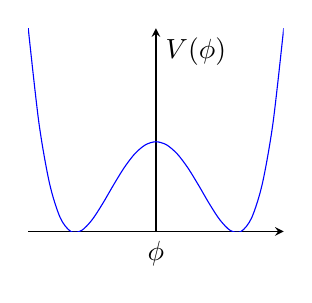
\begin{tikzpicture}
\begin{axis}[width=1.9in,axis x line=middle, axis y line=center, 
            ticks=none, xlabel= $\phi$, ylabel = $V(\phi)$,
            xlabel near ticks,
            ]
\addplot+[mark=none,smooth](\x,{(\x^2 - 10)^2});
\end{axis}
\end{tikzpicture}
\caption{The potential described in \eqref{eq:single_real_field_potential}, as a function of a spatially constant field $\phi$.}
\label{fig:single_real_field}
\end{marginfigure}
This Lagrangian is invariant under the reflection of the field, $\phi\rightarrow -\phi$. The Hamiltonian (density) $\mathcal{H}$ can be obtained by performing a Legendre transform:
\begin{align}
\mathcal{H} = \frac{\partial\mathcal{L}}{\partial\dot{\phi}}\dot{\phi} - \mathcal{L} = \frac{1}{2}(\partial_0\phi)^2+ \frac{1}{2}(\nabla\phi)^2+ V(\phi).
\end{align}
The quantity $\mathcal{H}$ corresponds to an energy density, with kinetic energy $\frac{1}{2}(\partial_0\phi)^2$ and potential energy $\frac{1}{2}(\nabla\phi)^2 + V(\phi)$. Since $(\nabla\phi)^2 \geq 0$, the minimum of this potential energy is achieved when $\nabla\phi = 0$, that is, the field must be a constant in space - let us denote this minimum constant value by $\phi_0$. The two possibilities for $\phi_0$ that minimize the potential in \autoref{fig:single_real_field} are $\phi_0 = \pm\sqrt{m^2/\lambda}$. The ground state of the theory must correspond to one of these.

Since it does not matter which minimum we choose, we can arbitrarily choose the positive value. This is known as the the \emph{vacuum expectation value} (\textsc{vev}). Having chosen this minimum, we can rewrite our Lagrangian in terms of the field $\phi' = \phi - \sqrt{m^2/\lambda}$ (note that we can do this because the physics remains the same under this translational redefinition of the field):

\begin{align}
\mathcal{L}(\phi') = \frac{1}{2}\partial^\mu\phi'\partial_\mu\phi' - V_\text{eff}(\phi')\\
V_\text{eff}(\phi') = \frac{\lambda}{4} + \sqrt{\frac{m^2}{\lambda}}\phi'^3 + m^2\phi'^2
\label{eq:potential_hidden_symmetry}
\end{align}
\begin{marginfigure}
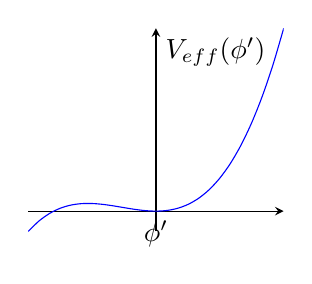
\begin{tikzpicture}
\begin{axis}[width=1.9in,axis x line=middle, axis y line=center, 
            ticks=none, xlabel= $\phi'$, ylabel = $V_\text{eff}(\phi')$,
            xlabel near ticks,
            ]
\addplot+[mark=none,smooth] {10*x^3 + 40*x^2};
\end{axis}
\end{tikzpicture}
\caption{The potential (\eqref{eq:potential_hidden_symmetry}) `seen' by the ground state, as a function of a spatially constant field $\phi'$.}
\label{fig:hidden_symmetry}
\end{marginfigure}

This Lagrangian is no longer symmetric under reflection, i.e. it is not invariant under the transformation $\phi'\rightarrow -\phi'$. This potential is minimized at $\phi' = 0$, which is convenient for performing perturbation theory. The mass of physical particles corresponding to quantum fluctuations of this vacuum is given by $V''_\text{eff}~|_{\phi' = 0} = \sqrt{2}m$. Note that we have not done anything to the system to break this symmetry. The symmetry of the original Lagrangian is contained in the relationships between the coefficients of the terms of the new Lagrangian. Keeping the above in mind, it might be more helpful to think about the symmetry as being \emph{hidden} by choosing a particular \textsc{vev}.


\subsection{Single complex field}

What if the field $\phi$ was complex, instead of real? It would then have an additional degree of freedom, contributed by its imaginary component. This makes it possible for the Lagrangian to have a continuous symmetry, as opposed to the discrete reflection symmetry in the previous example. The potential has the same general structure:
\begin{align}
V(\phi) = \frac{\lambda}{4}\left(\phi^{*}\phi - \frac{m^2}{\lambda}\right)^2
\label{eq:single_complex_field_potential}
\end{align}

\begin{marginfigure}
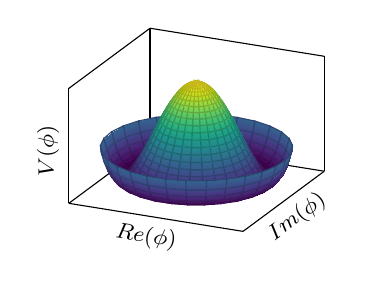
\begin{tikzpicture}
\begin{axis}[
			xlabel=$Re(\phi)$,
			ylabel=$Im(\phi)$,
			zlabel=$V(\phi)$,
            ticks=none,
			colormap name = viridis,
            xlabel style={sloped like x axis, font = \footnotesize},
            ylabel style={sloped like y axis, font = \footnotesize},
            zlabel style={font = \footnotesize},
			width=1.9in,
            samples=30,
            domain=0:360,
            y domain=0:1.25,
        ]
        \addplot3 [surf, 
					shader=faceted interp,
				   z buffer=sort] ({sin(x)*y}, {cos(x)*y}, {(y^2-1)^2});
        \end{axis}
\end{tikzpicture}
\caption{The infamous `Mexican hat potential.}.
\end{marginfigure}

In this case, the Lagrangian has an additional symmetry, known as
global U(1) symmetry. This means that it is invariant under transfor- mations of the form $\phi\rightarrow e^{i\theta}\phi$ where $\theta$ is a parameter independent of space-time. The form of transformation suggests rotations, and indeed we can see that this potential will be invariant under rotations about its symmetry axis \footnote{ The reflection symmetry from the previous example is incorporated here - it is nothing but a U(1) transformation with $\theta = \pi$.}.

We can pick any of the points at the minimum of this potential as a vacuum expectation value. To recover a similar scenario as the previous example, we can pick $\phi_0 = \sqrt{m^2/\lambda}$. This reproduces a theory with a particle of mass $\sqrt{2}m$.

You can imagine the potential as a surface along which a ball rolls, and the the mass to be analogous to the `resistance' the ball faces from the surface it if tries to roll. This resistance is given by the curvature of the surface - the second derivative of the potential function.
At $\phi = 0$ there is `negative resistance', corresponding to tachyons with imaginary mass, whereas if it resides in one of the troughs, then it would face some resistance, corresponding to particles with positive mass.

We see that the curvature in the radial direction will provide some resistance, but there is no curvature in the angular direction - the ball can roll around in a circle without any resistance. Since the curvature in the angular direction is zero, the mass of the particle will be zero.

Basically, we can write our single complex field in terms of two real fields, one corresponding to the radial degree of freedom and the other corresponding to the angular degree of freedom. We can interpret these two real fields as particles. The field that can only change in the radial direction now has positive mass, whereas the field that can change in the angular direction is massless. This field corresponds to a massless particle, termed the Goldstone boson.

In fact, this is but an example of a more general result known as \emph{Goldstone's theorem}, which states that for every spontaneous breaking of a continuous symmetry, there appears a set of massless scalar bosons corresponding to the generators of the symmetry group.

\subsection{Local U(1) symmetry}

We have already seen in \autoref{sec:gauge_invariance} an example of the ramifications of an unbroken $U(1)$ gauge symmetry, which led to a structure very much like \textsc{qed}. Let us now see what happens when this symmetry is spontaneously broken. Our Lagrangian is the same as that for but now invariant under transformations of the form $\phi\rightarrow e^{i\theta(x)}$, where $\theta(x)$ is a function of space and time.  Like before, we promote the partial derivatives $\partial_\mu$ to covariant derivatives $\partial_\mu - igA_\mu$, where the vector field $A_\mu$ transforms as $A_\mu + \frac{1}{g}\partial_\mu\theta(x)$. Our Lagrangian now reads
\begin{align}
\mathcal{L}(\phi) &= \frac{1}{2} D^\mu\phi D_\mu\phi - V(\phi)-\frac{1}{4}F_{\mu\nu}F^{\mu\nu}\\
V(\phi) &= \lambda\left(\phi^*\phi - \frac{v^2}{2}\right)^2
\end{align}
where $v = \sqrt{\mu^2/\lambda}$. We can now proceed with spontaneously breaking this symmetry. To do so, we choose a vacuum expectation value $\langle\phi\rangle = v/\sqrt{2}$ If we write our original complex field as $\phi = e^{i\xi(x)/v}(v+\rho(x))/\sqrt{2}$, where $\xi(x)$ and $\rho(x)$ are two real fields corresponding to the angular and radial degrees of freedom respectively. When we pick the vacuum expectation value $v/\sqrt{2}$, this sets $\langle\xi\rangle = \langle\rho\rangle=0$. We can then write the Lagrangian in terms of $\xi$ and $\rho$ as follows:

\begin{equation*}
\mathcal{L}(\xi,\rho) = \frac{1}{2}\partial_\mu\rho\partial^\mu\rho + \frac{(v + \rho)^2}{2}%
\left(-gA_\mu+\frac{\partial_\mu\xi}{v}\right)^2-\frac{\lambda}{4}\left(\rho^2 + 2v\rho^2\right)^2%
-\frac{1}{4}F_{\mu\nu}F^{\mu\nu}
\end{equation*}
In this form, we see that there is a mass term of the form $A_\mu A^\mu$ for the gauge field. However, there is also a mixed term, $-gvA_\mu\partial^\mu\xi$ whose interpretation is not immediately clear. We can fix this by choosing a gauge, known as the \emph{unitary gauge} that makes $\phi$ always real:
$\theta(x) = \frac{\xi(x)}{gv}$
When we do so, the terms with $\xi$ disappear. Thus, gathering the terms in the Lagrangian quadratic in the fields, we get
\begin{equation}
\mathcal{L}_\text{quadratic}^\text{unitary gauge} = \frac{1}{2}\partial_\mu\rho\partial^\mu\rho + g^2v^2 A_\mu A^\mu - \lambda v^2\rho^2 - \frac{1}{4}F_{\mu\nu}F^{\mu\nu}
\end{equation}
We see that the field $A_\mu$ acquires a mass of $gv$ and the field that changes along the radial direction, $\rho$, acquires a mass as well. We term this field the physical \emph{Higgs boson}. We seem to have gotten rid of the Goldstone boson that should appear due to Goldstone’s theorem! However, upon closer inspection, we see that the Goldstone boson is just hidden in the theory as an extra degree of freedom. After symmetry breaking, the massless gauge field combines with one of the scalar fields to form a massive vector field. We can shed some light on the situation by examining the degrees of freedom. The gauge field originally had two degrees of freedom corresponding
to the two possible polarization states, and the $\xi$ and $\rho$ had one degree of freedom each. The $\rho$ retained its degree of freedom, but the vector boson field now has three degrees of freedom (three possible polarization states) after `eating' the $\xi$ field. The $\xi$ field is called a `would-be' Goldstone boson. We have just finished describing the Higgs mechanism for the spontaneous breaking of an Abelian symmetry. Having performed these warm-up exercises, we are in good shape to tackle electroweak symmetry breaking.


\section{Electroweak symmetry breaking}

Electroweak symmetry breaking is the spontaneous breakdown of the product group $SU(2)_L\times U(1)_Y\rightarrow U(1)_{EM}$. This is achieved by adding to the theory a scalar field $H$:
$$H = \vdoublet{H^+}{H^0}$$
The terms of the Lagrangian that involve this field can be written as follows:
\begin{align}
  \label{eq:higgs_kinetic}
  \mathcal{L}_{\text{Higgs}} &= \frac{1}{2}\left|D_\mu H\right|^2-V(H)\\
  \label{eq:higgs_potential}
  V(H) &= \left(H^\dag H-\frac{v^2}{2}\right)^2
\end{align}
where $v = \sqrt{\frac{\mu^2}{\lambda}}$. Since we have three generators $(T_a)$ for the $SU(2)$ symmetries, and one $(Y)$ for the $U(1)$ symmetry, we will introduce four gauge fields to construct the covariant derivative $D_\mu$.
\begin{align*}
  SU(2)&\rightarrow W_\mu^1,W_\mu^2, W_\mu^3\\
  U(1)&\rightarrow B_\mu
\end{align*}
Thus the gauge covariant derivative takes the form
$$D_\mu = \partial_\mu + igW_\mu^a\frac{\tau^a}{2}+ig'YB_\mu.$$
The potential $V(H)$ reaches its minimum when $H^\dag H = v^2 / 2$. We pick a vacuum expectation value for $H$ that breaks the neutral sector symmetry (corresponding to $H^0$) but not the charged symmetry (corresponding to $H^{+}$), since we wish to keep photons massless. Thus, we can pick the \textsc{vev}:
$$H = \vdoublet{0}{\frac{v}{\sqrt{2}}}$$
Plugging this into the kinetic term of the Lagrangian gives us:
\begin{align*}
  (D_\mu H)^\dag(D_\mu H) &= \begin{pmatrix} 0 & \frac{v}{\sqrt{2}}\end{pmatrix}
  \left(\partial_\mu - igW_\mu^a\frac{\tau^a}{2}
  -\frac{ig'}{2}B_\mu\right)
  \left(\partial_\mu+igW_\mu^a\frac{\tau^a}{2}+\frac{ig'}{2}B_\mu\right)
  \vdoublet{0}{\frac{v}{\sqrt{2}}}
\end{align*}
If we simplify the above expression and isolate the terms quadratic in the gauge fields, we get
\[\frac{g^2v^2}{4}W_\mu^-W_\mu^++\frac{1}{2}\frac{v^2}{4}(g^2+g'^2)
\left(\ct W_\mu^3 - \st B_\mu\right)^2\]
where $W_\mu^\pm = (W_\mu^1\pm iW_\mu^2)/\sqrt{2}$  and $\theta_w = \tan^{-1}(g'/g)$ is the \emph{Weinberg angle}, which parameterizes the mixing between the photon $A_\mu$ and the $Z$ boson.
\begin{equation}\label{eq:z_a_mixing}
\vdoublet{Z_\mu}{A_\mu} = \fourmatrix{\ct}{-\st}{\st}{\ct}
\vdoublet{W_{\mu}^{3}}{B_{\mu}}
\end{equation}
\subsection{Mass generation for \emph{W} and \emph{Z} bosons}
The product $W_\mu^+W_\mu^-$ can be interpreted as a mass term for a generic charged vector boson $W_\mu^\pm$. Rewriting our mass terms for the vector boson fields with the above redefinitions, we get
\[\mathcal{L}_{\text{mass terms}}=\frac{e^2v^2}{4\sin^2\theta_w}W_\mu W^\mu+
\frac{e^2v^2}{8\sin^2\theta_w\cos^2\theta_w}Z_\mu Z^\mu\]
After accounting for symmetry factors, we get the masses of the W and Z bosons as:
\begin{align*}
  m_W &=\frac{ev}{2\st} & 
  m_Z &=\frac{ev}{\sin2\theta_w}
\end{align*}
We see that there is no mass term for $A_\mu$, which means that this gauge field remains massless. Thus we see that the W and Z bosons gain mass, limiting their range, while the photon remains massless, corresponding to what is experimentally observed. 

\subsection{Fermion mass generation}

Till now we have not addressed the question of fermion masses in a chiral theory. In the Dirac Lagrangian, we had a mass term for the fermion field of the form $m\bar{\psi}\psi$. However, we found out that a Dirac spinor is in fact a combination of left- and right-handed Weyl spinors. If we write the mass term using Weyl spinors, we would have
$$m(\bar{\psi_L}\psi_R+\bar{\psi_R}\psi_L)$$
It is experimentally observed that weak interactions break parity, that is, they treat left- and right-handed fields differently. This means that the term above, while Lorentz-invariant, is not gauge invariant under the $SU(2)_L$ gauge symmetry, and is thus forbidden. Conveniently, the Higgs mechanism fixes this problem as well.

Fermion masses can be generated by their coupling to the Higgs doublet $H$. Terms such as $-y\bar{L}H\psi_R$, where $y$ is a dimensionless coupling constant, are gauge-invariant. This type of coupling is known as a \emph{Yukawa coupling}. After electroweak symmetry breaking, the Higgs field acquires a \textsc{vev}, and the above term becomes
\begin{equation}\label{eq:fermion_masses}
-\frac{yv}{\sqrt{2}}\bar{\psi}_L\psi_R
\end{equation}
where $yv/\sqrt{2}$ is the mass of the fermion. In general, the masses of fermions are proportional to their Yukawa couplings.

\section{Electroweak Interactions}

The interactions between fermions and the electroweak vector bosons ($W,Z,\gamma$) can be derived by inspecting the kinetic terms of the fermions:
\begin{equation}
  i\bar{L}\slashed{D}L + i\bar{\psi_R}\slashed{D}\psi_R + i\bar{\psi'_R}\slashed{D}\psi'_R
\label{eq:interaction_lagrangian}
\end{equation}
Here, $L$ is a fermion doublet of the form
$$L = \vdoublet{\psi'_L}{\psi_L}$$
The pair of fields $(\psi', \psi)$ can be one among the following: 
$$(\nu_e,e), (\nu_\mu,\mu), (\nu_\tau, \tau), (u, d), (c, s), (t, b)$$
However, the third term in \eqref{eq:interaction_lagrangian} would not exist for the first three pairs listed above, since right-handed neutrinos have not been experimentally found\footnote{Although we do know now that neutrinos have mass, and the existence of a as-yet heavy undetected right-handed neutrino is a possible mechanism for generating neutrino masses.}. The subscripts \emph{L} and \emph{R} denote the handedness of the fields.
\subsection{Charged currents}
We will first consider the charged currents, corresponding to interactions involving $W^\pm$. To do this, we will isolate the terms in the covariant derivative $D_\mu$ that correspond to them, that is, the terms containing $W_1^\mu$ and $W_\mu^2$. Writing this out, we get terms of the form:
\begin{equation*}
  -\frac{g}{\sqrt{2}}\bar{\psi'_L}\gamma^\mu W_\mu^+\psi_L + \text{h.c}.
\end{equation*}
\begin{marginfigure}
\feynmandiagram [vertical = w to v] {
  f1 [particle = \(\psi_L\)] -- [anti fermion] v -- [boson] w [particle = \(W^\pm\)],
    f2 [particle = \(\psi'_L\)] -- [fermion] v,
};
\caption{Feynman diagram representing the weak charged current.}
\end{marginfigure}
These give us Feynman diagram vertices for the interactions mediated by W bosons.
\subsection{Neutral currents}
We can apply a similar treatment to the neutral gauge particles $A_\mu$ and $Z_\mu$. After performing the redefinition in \eqref{eq:z_a_mixing} and isolating the kinetic terms coupling these fields to the fermions in the Lagrangian, we get terms of the form
\[\bar{\psi}A_\mu(g\st T_3 + g'\ct Y)\psi+\bar{\psi}Z_\mu(g\ct T_3 - g'\st Y)\psi\]
Here, $\psi$ can be a left- or right-handed field. Remembering our previous definitions of $g$ and $g'$ in terms of the mixing angle $\theta_w$, we can write the expressions for $Z_\mu$ and its orthogonal field $A_\mu$.
The above expression can be simplified futher by noting that
$$g\st = g'\ct = \frac{gg'}{\sqrt{g^2 + g'^2}}.$$
We know that the strength of the electromagnetic interaction depends on the magnitude of the electric charge. Keeping this in mind, we relabel the constant $gg'/\sqrt{g^2 + g'^2}$ as $e$, the magnitude of the electric charge of the electron, and the operator $T_3 + Y$ as $Q$, whose eigenvalues correspond to the electric charge. 
So our neutral current terms become
$$e\bar{\psi}A_\mu Q\psi+ \bar{\psi}Z_\mu\frac{2e}{\sin 2\theta_w}(T_3 - \sin^2\theta_w Q)\psi$$

The different charges of the SM fermions under the operators $T_3, Y$, and $Q$ are given in \autoref{tab:charges}.
\begin{marginfigure}
\feynmandiagram [vertical = w to v] {
  f1 [particle = \(\psi_L\)] -- [anti fermion] v -- [boson] w [particle = {\(Z,\gamma\)}],
    f2 [particle = \(\psi_L\)] -- [fermion] v,
};
\caption{Feynman diagram representing the weak neutral and electromagnetic currents.}
\end{marginfigure}

\begin{margintable}
  \centering
  \begin{tabular}{lrrr}
    Field & $T_3$ & $Y$ & $Q$ \\
  \hline
  $\nu_L$   &  $\slantfrac{1}{2}$   & -$\slantfrac{1}{2}$   & 0\\
  $l_L$     & -$\slantfrac{1}{2}$   & -$\slantfrac{1}{2}$   & -1\\
  $l_R$     &        0              &                  -1   & -1\\
  $u_L$     &  $\slantfrac{1}{2}$   &   $\slantfrac{1}{6}$  & $\slantfrac{2}{3}$\\
  $u_R$     &        0              &   $\slantfrac{2}{3}$  & $\slantfrac{2}{3}$\\
  $d_L$     &        0              &                  -1   & -$\slantfrac{1}{3}$\\
  $d_R$     &  -$\slantfrac{1}{2}$  &   $\slantfrac{1}{6}$  & -$\slantfrac{1}{3}$\\
  \end{tabular}
  \caption{Charges of the various fields. Here, we have grouped the fields as follows:
      $l \in \{e, \mu, \tau\}$,
      $\nu \in \{\nu_e,\nu_\mu, \nu_\tau\}$,
      $u\in\{u,c,t\}$,
      $d\in\{d,s,b\}$.}
  \label{tab:charges}
\end{margintable}

\subsection{Gauge boson self-interactions}

The self-interactions of the gauge bosons follow the structure discussed in \autoref{sec:non_abelian}, with the appropriate mixing factors and the structure constants for the $SU(2)$, the antisymmetric Levi-Civita tensor $\epsilon_{ijk}$.

\subsection{The Higgs boson and its couplings}

Peter Higgs was the first to postulate the existence of a physical \emph{Higgs boson} that could be produced by perturbing the vacuum. To see how this plays out, let us parameterize the Higgs doublet field as 
\[H = \frac{1}{\sqrt{2}}\exp\left(i\xi^a(x)\frac{\tau^a}{v}\right)\vdoublet{0}{v + h(x)}\]
where the  $\langle\xi\rangle=\langle h\rangle=0$. The simplest gauge choice is the unitary gauge, where $\xi(x)=0$. In this gauge, the potential $V(H)$ from \eqref{eq:higgs_potential} becomes:
\[V(H) = -\frac{1}{2}m_h^2 h^2 - \lambda vh^3 -\frac{1}{4}\lambda h^4\]
The field $h$ is the physical Higgs boson. It is the only fundamental scalar in the Standard Model, and was discovered in 2012, nearly 50 years after it was first predicted. The coefficient of the term quadratic in $h$ is its mass, $m_h = \sqrt{2}\mu$. This mass is a free parameter that had to be determined experimentally. The second and third terms in the above expression represent the trilinear and and quartic self-coupling of the Higgs boson:
\begin{align*}
\feynmandiagram [small, baseline = (v.base), horizontal = h3 to v] {
  {h1 [label = \(h\)], h2 [label = \(h\)], h3 [label=\(h\)]} -- [scalar] v,
};
= i6\lambda v
&&
\feynmandiagram [small, baseline = (v.base), horizontal = h1 to h2] {
  {h1 [label = \(h\)], h2 [label = \(h\)], h3 [label=\(h\)], h4 [label=\(h\)]} -- [scalar] v,
};
= -i6\lambda
\end{align*}
The coupling of the Higgs boson to the $W$ and $Z$ bosons can be seen by re-examining the kinetic term in \eqref{eq:higgs_kinetic} in the unitary gauge:
\[\mathcal{L}_K = \frac{1}{2}(\partial_\mu h)^2 + \left(m_W^2 W_\mu^+ W^{\mu-} + \frac{1}{2}m_Z^2Z_\mu Z^\mu\right)\cdot\left(1+\frac{h}{v}\right)^2\]
which gives us the interaction vertices
\begin{align*}
\feynmandiagram [small, baseline = (v.base), horizontal = h to v] {
  {wp [label = \(W^+\)], wm [label = \(W^-\)]} -- [boson] v -- [scalar] h [label = \(h\)],
};
= 2i\frac{m_W^2}{v}g^{\mu\nu}
&&
\feynmandiagram [small, baseline = (v.base), horizontal = h to v] {
  {z [label = \(Z\)], wm [label = \(Z\)]} -- [boson] v -- [scalar] h [label = \(h\)],
};
= 2i\frac{m_Z^2}{v}g^{\mu\nu}
\end{align*}
The coupling to the fermions can be found by looking at the fermion mass terms from \eqref{eq:fermion_masses} in the unitary gauge. Doing so, we get the interactions shown in \autoref{fig:higgs_fermion_coupling}, where $m_f$ is the mass of the fermion. Thus we see that the coupling of the Higgs boson is in general proportional to the mass of the particle it couples to. As expected, we do not see any tree-level couplings between the Higgs boson and photons, which are massless. 
\begin{marginfigure}
\begin{align*}
\feynmandiagram [small, baseline = (v.base), horizontal = h to v] {
  {f1 [label = \(f\)], f2 [label = \(f\)]} -- [fermion] v -- [scalar] h [label = \(h\)],
};
= -i\frac{m_f}{v}
\end{align*}
\caption{The coupling of the Higgs boson to fermions.}
\label{fig:higgs_fermion_coupling}
\end{marginfigure}


\section{CKM mixing}
When we discussed fermion masses, we glossed over an interesting feature of the SM: the distinction between the mass and the gauge eigenstates of the quarks, first hinted at by the Cabibbo angle introduced in \autoref{sec:pre_yang_mills}. While gauge eigenstates have well defined transformations under gauge groups, the physical particles that we observe at a collider will in fact be mass eigenstates. The two are related by the \emph{Cabibbo-Kobayashi-Maskawa} (\textsc{ckm}) mixing matrix:

\begin{equation}
  V_\text{CKM} =
  \begin{pmatrix}
    V_{ud} & V_{us} & V_{ub}\\
    V_{cd} & V_{cs} & V_{cb}\\
    V_{td} & V_{ts} & V_{tb}
  \end{pmatrix}
\end{equation}
This matrix has been experimentally determined to be nearly diagonal, with the elements getting smaller as they are further off-diagonal.

\section{Asymptotic freedom and QCD}
In the 50s and 60s, experiments were devised to unravel the structure of the proton. They found two seemingly incompatible results: on the one hand, colliding protons resulted in the production of a large number of pions collinear with the beam axis, implying that the protons could not absorb a large momentum transfer. However, deep inelastic scattering experiments showed that it was possible for an energetic electron to undergo hard electrmagnetic scattering off a proton. These disparate phenomena were reconciled by the introduction of the \emph{parton model} by Bjorken and Feynman. In this model, hadrons were comprised of a collection of loosely bound pieces, known as partons. To an energetic incoming electron, these partons would appear approximately free, allowing it to scatter with a large momentum transfer off of one of them. The struck parton will then exchange momentum softly via the strong interaction among the other partons, which results in the production of a \emph{jet} of hadrons, collinear with the direction of the original struck parton. The deeper reason for this behavior is that these partons are charged under a non-Abelian gauge group, $SU(3)$. The phenomenon of the weakening of the strong interaction at large momentum transfers is known as \emph{asymptotic freedom}, and it is a property of non-Abelian gauge theories.

The $\beta$-function of a gauge theory describes the evolution of the coupling constant with energy. For non-Abelian gauge theories, it takes the following form (up to leading order):
\begin{equation}
  \beta(g_R) = \mu\frac{d}{d\mu}g_R = -\frac{g_R^3}{(4\pi)^2}\left[\frac{11}{3}C_A -\frac{4}{3}n_fT_F\right]
\end{equation}
where $\mu$ is the renormalization scale, $C_A$ is the quadratic Casimir operator for the adjoint representation, and $T_F$ is the \emph{index} of the fundamental representation.
In the case of the strong interaction, the relevant gauge group is $SU(3)$. Thus $C_A = 3$ and $T_F = \frac{1}{2}$. If $n_f$, the number of quark flavors is less than 17 \footnote{Which it is, since the number of quark flavors is six, as can be seen in \autoref{tab:quarks}.}, the $\beta$ function has a \emph{negative} sign, which means that the coupling \emph{decreases} at higher energies. This is the underlying basis of asymptotic freedom. The theory of the strong interaction is known as \emph{quantum chromodynamics}, or QCD for short. The analogue of electric charge for this theory is a quantity referred to as \emph{color} (hence the name of the theory). The gauge fields that mediate this interaction, that correspond to the generators of $SU(3)$, are known as \emph{gluons}. At a hadron collider, it is of crucial importance to understand the physics of gluons and jets.
\begin{marginfigure}[-15cm]
  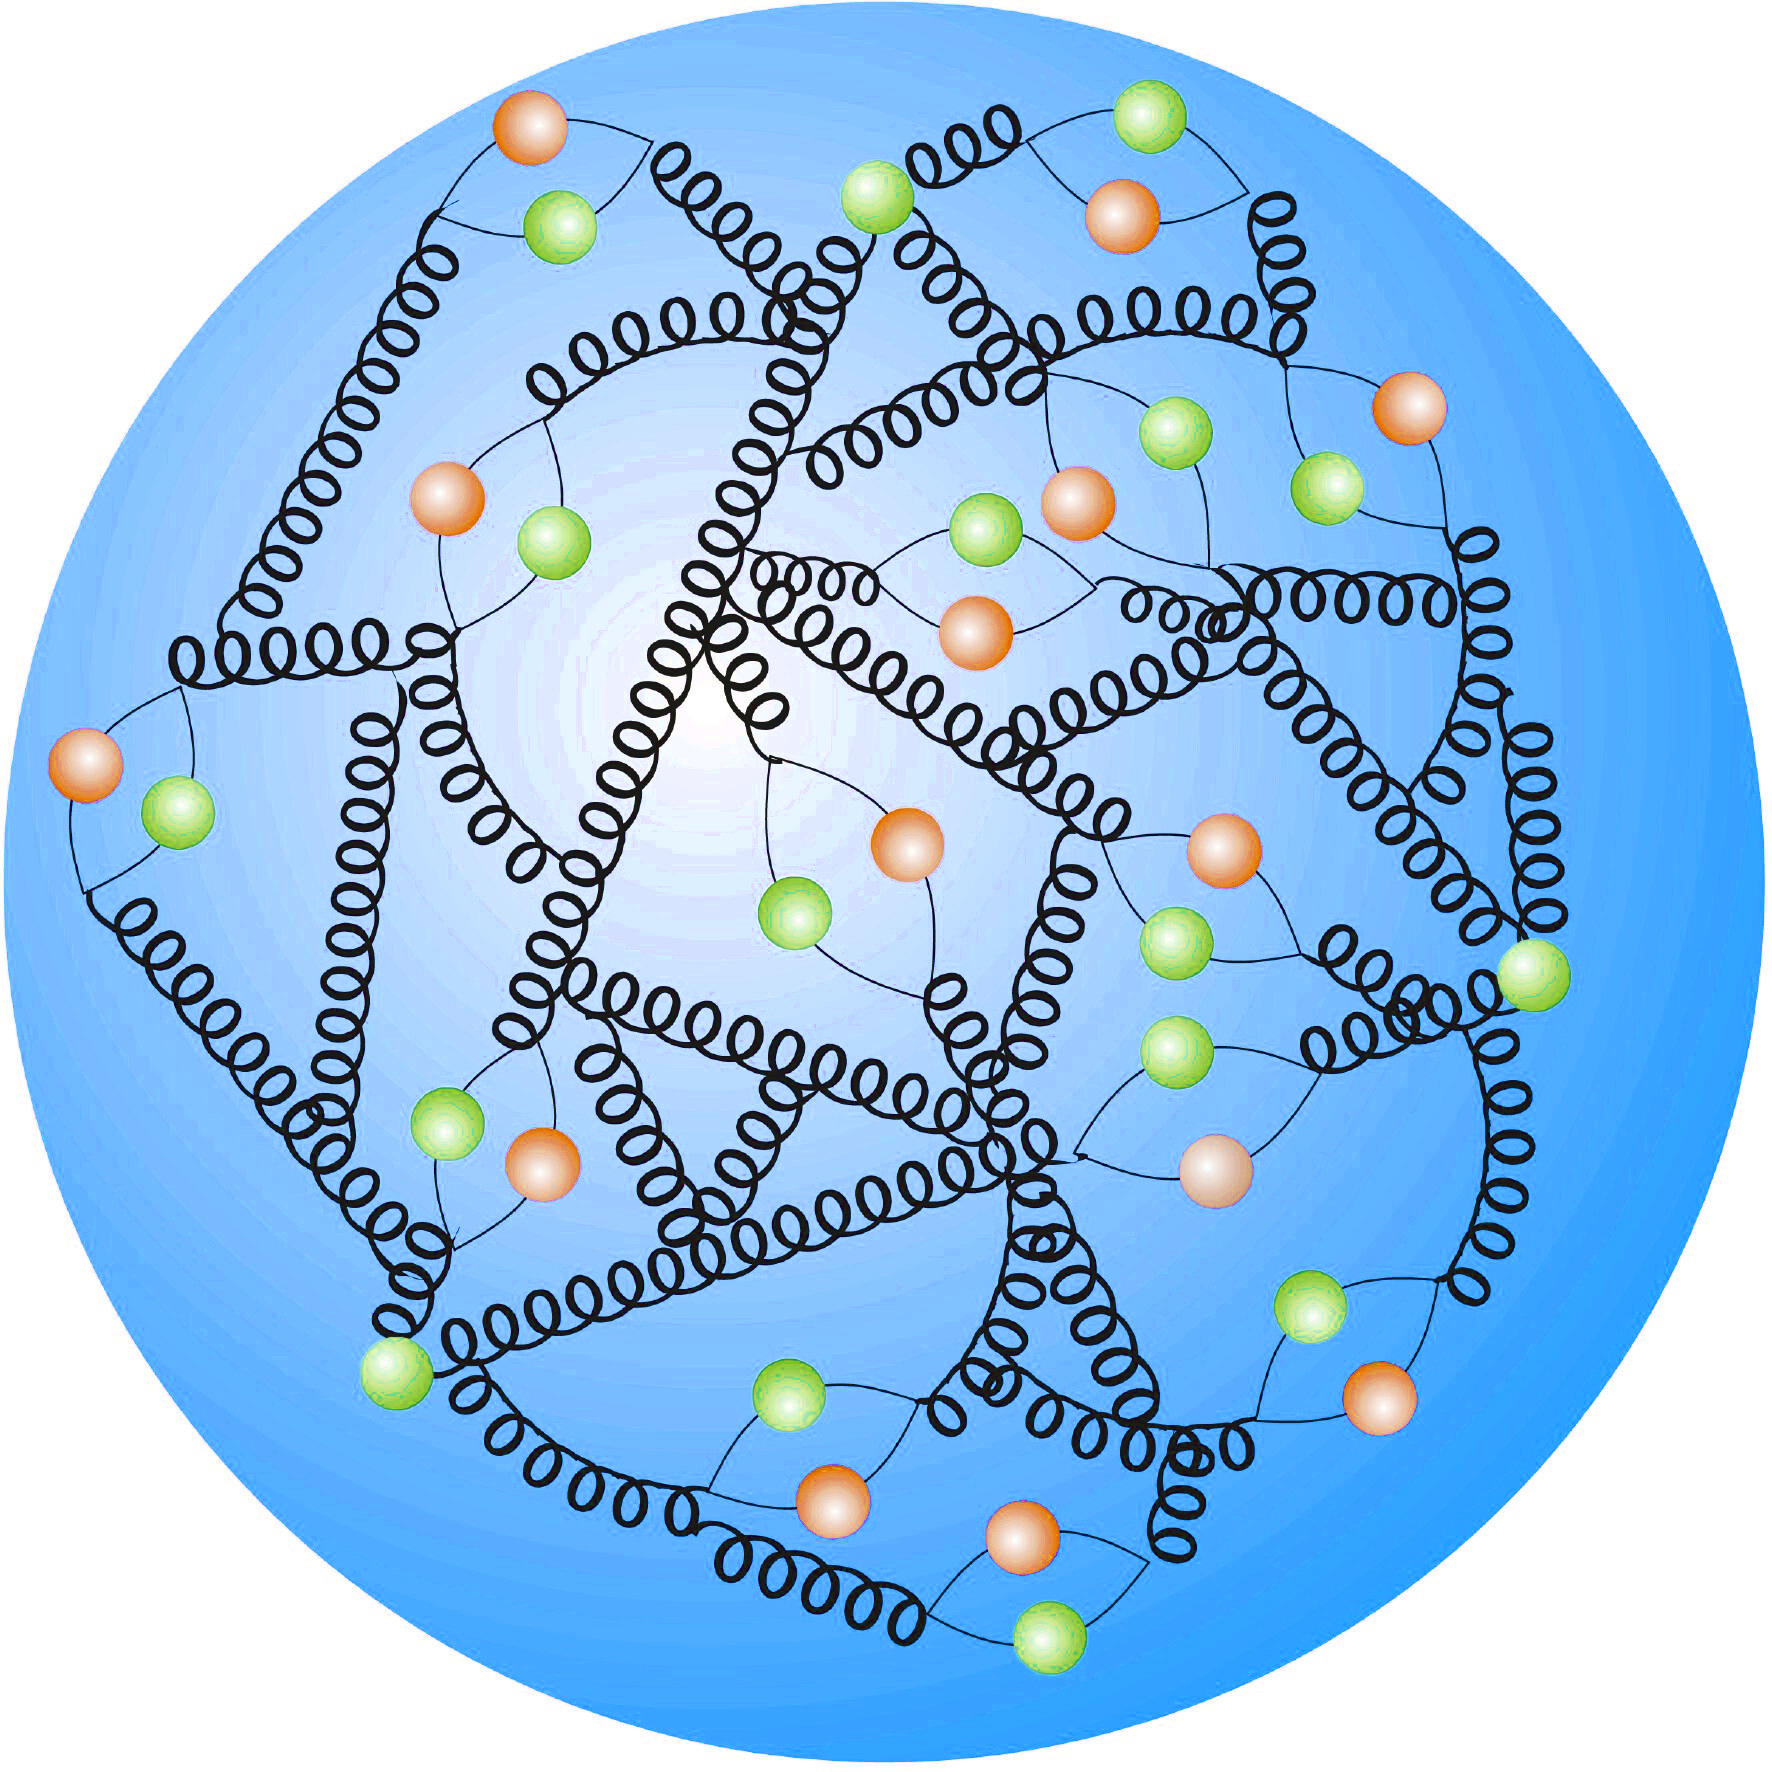
\includegraphics[width=0.8\textwidth]{images/proton_innards}
\caption{A representation of the innards of a proton, showing the dynamic structure. Image source:\citep{proton_structure}}
\end{marginfigure}

\section{Limits of the Standard Model}
The Standard Model of particle physics has been remarkably successful, and over the decades has yielded some of the most precise measurements in all of physics. However, as mentioned in \autoref{ch:introduction}, there still remain unresolved issues with the SM. Some of the more pressing ones include the following.

\paragraph{Quantum Gravity} So far, we have seen that the SM explains the electromagnetic, weak, and strong interactions. As it turns out, gravity can be cast as a quantum field theory as well, with the gravitational force mediated by spin-2 particles known as \emph{gravitons}. The trouble is that, like Fermi's theory of weak interactions, it is a non-renormalizable theory, valid only much below the Planck scale. Just as Fermi's theory was shown to be a low-energy effective approximation for the Glashow-Weinberg-Salam theory of weak interactions, it is believed that quantized general relativity is similarly a low-energy approximation to some underlying theory that is perturbative at the Planck scale as well. The pre-eminent contender for a perturbative theory of quantum gravity is \emph{string theory}, which describes particles as strings of finite size that propagate through space-time and interact with each other. Another approach is based upon discretizing space-time itself, and is known as \emph{loop quantum gravity}.

\paragraph{Neutrino masses} Experiments have shown that neutrinos have a small mass, in conflict with the Standard Model, which predicts massless neutrinos. There have been a number of proposed extensions to the Standard Model that address this issue.
\paragraph{Hierarchy problem}
The hierarchy problem, which we will return to in \autoref{ch:supersymmetry},  refers to the troubling sensitivity of the mass of the Higgs to any new physics at higher energy scales - the parameters of any new physics theory must be extremely \emph{finely-tuned} to recover the experimental value of the Higgs mass that is observed.
\paragraph{Baryon asymmetry} The SM by itself does not explain the magnitude of the imbalance between matter and antimatter in the universe. We need some additional mechanism to do so.
\paragraph{The strong CP problem} While the weak interactions violate parity, we observe that the strong interactions do not. However, it is possible to write a term in the Lagrangian that is CP-violating, but this term is vanishingly small. There is no a priori reason that this term must be so small, and thus it is an another example of a fine-tuning problem, similar to the hierarchy problem discussed previously, and is known as the \emph{strong CP problem}.
\paragraph{Dark Matter}
Experiments have shown that visible matter accounts for only a small fraction of the universe. The majority consists of \emph{dark energy} and \emph{dark matter}. The SM has no viable dark matter candidate, and clearly needs to be augmented to satisfactorily incorporate dark matter.

Clearly there is much motivation to come up with extensions to the Standard Model. In the next two chapters, we will discuss two kinds of extensions to the Standard Model: Two-Higgs Doublet Models, and supersymmetric models. More specifically, we will describe the salient features of the Minimal Supersymmetric Standard Model, or MSSM.
